\subsection{Nanowire with localized curvature gradient} \label{subsec:Parabolic_wire}

Magnetic properties of ferromagnetic elements at the nanoscale are governed not only by the intrinsic material properties, but also by geometries of elements. This dependence manifests itself during the motion of magnetization textures and their magnetic responses to the external influences. Thus, the appropriately engineered geometry of magnetic elements can introduce additional local energy minima in a small magnetic structures, which can for instance be set to a multidomain state due to the magnetostatic interaction that favors magnetization alignment along the element edges. These can result in a reproducible and controlled formation of domain walls in magnetic curvilinear geometries. The behavior of domain walls in planar curvilinear magnetic nanowires is a topic of great technological interest due to their perspective application in modern memory~\cite{Hayashi07,Parkin08} and logic devices~\cite{Allwood02,Allwood04,Allwood05,Hayashi08}. The suitability of domain walls for these application originate from their topological stability and particle-like properties, which allow them to be assigned as an information carrier in a similar manner to charge signals in conventional microelectronic systems~\cite{Klaui08,Jiang11,Negoita12}. The modification of dynamics and static properties of a domain wall due to the wire curvature is of high importance for the application, due to the influence of localized curvilinear defects on the appearance of pinning potential for domain walls~\cite{Lewis09,Glathe12,Burn14}. This means that changes in local geometrical shapes engineer the energetic landscape, that can be utilized for the precise positioning of domain walls. 

\subsubsection{Domain walls in parabolic nanowire} \label{subsubsec:Parabola_theory}

To demonstrate the influence of the exchange-induced chiral effects on magnetic domain walls in nanowire with localized curvature, we will consider here the case of parabolic wire geometry:
\begin{equation} \label{eq:parabola_wire}
	\vec{\gamma} = x \, \hat{\vec{x}} + \dfrac{\kappa_0 \, x^2}{2} \, \hat{\vec{y}},
\end{equation}
which is the mathematically simplest possible curve with well-defined geometry and curvature distribution:
\begin{equation}
	\kappa = \dfrac{\kappa_0}{(1+\kappa^2_0 \, x^2)^{3/2}}.
\end{equation}  

For the further analysis it is convenient to rewrite the total micromagnetic energy~\eqref{eq:total_energy} in the normalized form, $\mathcal{E} = E/4 \, \pi \, M_s^2$, by using the angular magnetic parameterization $\vec{m} = \cos\theta \, \vec{e}_{\textrm{T}}+\sin\theta \, \cos\phi \, \vec{e}_{\textrm{N}} + \sin\theta \, \sin \phi \, \vec{e}_{\textsc{B}}$, 
\begin{equation}\label{eq:Parabola_total_energy}
	\begin{split}
		\mathcal{E} &= S \, \int^{+ \infty}_{-\infty}\mathrm{d}\vec{s} \, \left[\ell^2 \, (\theta' + \kappa \, \cos \phi)^2 + \ell^2 (\phi' \, \sin \theta  - \kappa \, \cos \theta \, \sin \phi)^2 -k_t \, \cos^2 \theta \right],
	\end{split}
\end{equation}
where $S$ is the area of the wire cross section, $\ell = \sqrt{A/(4 \, \pi \, M^2_s)}$ is the exchange length and $k_t = K/(4 \, \pi \, M^2_s) + 1/4$ is the dimensionless anisotropy constant. The equilibrium magnetic state for \eqref{eq:Parabola_total_energy} could be determined by means of the energy minimization technique, which results in a planar solution with $\phi = \phi_0 = 0, \, \pi$ and $\theta$ determined by an inhomogeneous Sine-Gordon equation 
\begin{equation} \label{eq:Parabola_theta_equation}
	\ell^2_m \, \theta'' - \sin \theta \, \cos \theta = - \ell^2_m \, \kappa' \, \cos \phi_0,
\end{equation}
where $\ell_m = \ell/\sqrt{k_t}$ is the magnetic length.

For the case $\kappa' = 0$, which takes place in rectilinear and circular wires, the Eq.~\eqref{eq:Parabola_theta_equation} has a well known domain wall solution $\cos \theta = - p \, \tanh[(s-q)/\Delta]$, where $p$ is the domain wall polarity: $p=1$ for head-to-head and $p=-1$ for tail-to-tail domain walls, respectively. Here $q$ determines the domain wall position along the wire and $\Delta = \ell_m$ is the wall width. For the case $\kappa' \neq 0$ an additional driving force appears and the curvature-induced domain wall dynamics is expected. 

To analyze the domain wall properties, it is instructive to use a collective variable approach~\cite{Slonczewski72,Thiele73} based on the simple $q$ -- $\Phi$ model~\cite{Slonczewski72,Malozemoff79} 
\begin{equation} \label{eq:q-phi_model}
	\cos \theta = - p \, \tanh \left[ \dfrac{s-q(t)}{\Delta} \right], \qquad \phi = \Phi(t).
\end{equation}
The domain wall position $q$ and phase $\Phi$, which determines orientation of the transversal magnetization component, make a cononically conjugated pair of collective variables. Substituting the model Ansatz \eqref{eq:q-phi_model} to \eqref{eq:Parabola_total_energy} one obtains the resulting energy of the domain wall~\cite{Yershov15b}
\begin{equation} \label{eq:DW_total_energy}
	\dfrac{\mathcal{E}}{2 \, S} = \left( \dfrac{\ell^2}{\Delta} + k_t \, \Delta \right) + \pi \, p \, \ell^2 \, \kappa(q) \, \cos\Phi - \ell^2 \, \kappa^2(q) \, \Delta \, \sin^2 \Phi,
\end{equation}
where the condition $\kappa \, \Delta \ll 1$ was applied during the integration. The first term in \eqref{eq:DW_total_energy} corresponds to the interplay between exchange interaction and magnetic anisotropy, which determines the domain wall width similar to the case of a rectilinear wire. The second and the third terms are curvature-induced exchange-driven effective DMI-like and anisotropy-like terms~\cite{Yershov15b,Sheka15}. Minimization of the total energy of the domain wall \eqref{eq:DW_total_energy} with respect ot collective variables $q$ and $\Phi$ results in the following equilibrium values $q_0$ and $\Phi_0$:
\begin{equation} \label{eq:qPhi_equilibrium}
	\kappa'(q_0) = 0, \qquad \cos \Phi_0 = -p.
\end{equation} 
The exchange-driven effective DMI leads to the reshaping of the domain wall total energy \eqref{eq:DW_total_energy} in a way of appearance additional potentials corresponding to the type of domain walls: (i) In the case of two transversal domain walls with $p=+1$, $\Phi=\pi$ (head-to-head) and with $p=-1$, $\Phi=0$ (tail-to-tail) the curvature-induced DMI form a potential well at the apex region, see Fig.~\ref{fig:Parabola_n_straight_DWs}(a). (ii) In the case of two other possible configuration of transversal domain walls with $p=+1$, $\Phi=0$ (head-to-head) and with $p=-1$, $\Phi=\pi$ (tail-to-tail), there is a potential wall, see Fig.~\ref{fig:Parabola_n_straight_DWs}(b).  This is in contrast to a straight stripe system, where all four possible types of transversal DWs are energetically equal and stable in a sense of neutral equilibria in the $q$ -- $\Phi$ model framework, see Fig.~\ref{fig:Parabola_n_straight_DWs}(c).

%==================================================================\
%\begin{figure}[t]
%	\center{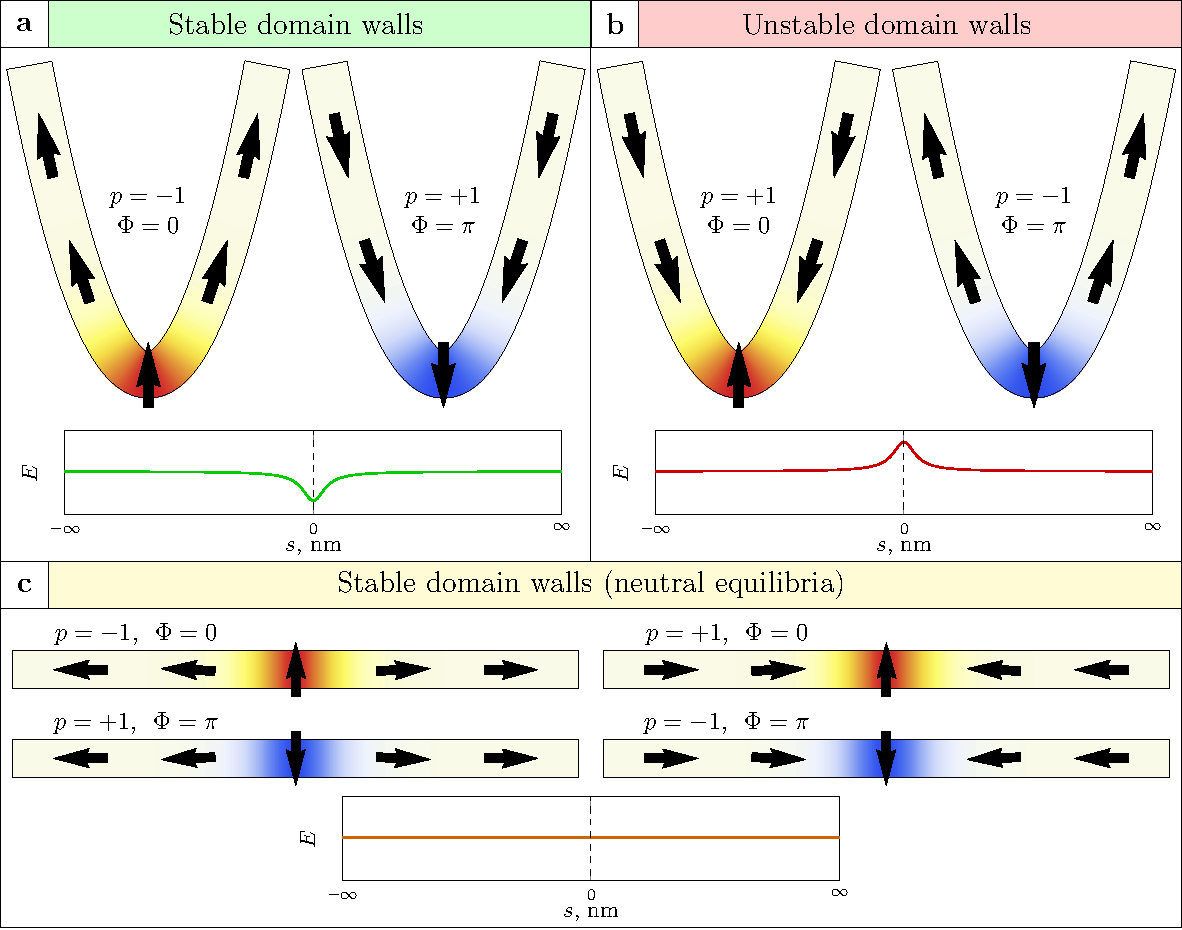
\includegraphics[width=0.9\linewidth]{Parabola_n_straight_stripe_sketch_SupplMat_1}}
%	\caption{\textbf{Curvature-induced asymmetrical stability of transversal DWs and their comparison with similar DWs in straight stripes.} \textbf{(a)},~Stable tail-to-tail and head-to-head DWs and their energy landscape on DWs position along the parabolic stripe. The energy landscape is calculated by means of the $q$ -- $\Phi$ model. The potential well at the apex region appears due to the influence of the curvature-induced DMI. \textbf{(b)},~Unstable head-to-head and tail-to-tail transversal DWs in a parabolic stripe and corresponding to them potential wall. \textbf{(c)},~Transversal DWs in a straight stripe, with their neutral stability within the framework of the $q$ -- $\Phi$ model. Adapted with permission from~\cite{Volkov19c}.}
%	\label{fig:Parabola_n_straight_DWs}
%\end{figure}
%==================================================================/

As it follows from~\eqref{eq:q-phi_model}, the equilibrium value of the domain wall width $\delta_0 = \ell_m$ is the same as for a straight wire. However, if the wall is not in the equilibrium position and the collective variables $(q,\Phi)$ deviate from the equilibrium \eqref{eq:qPhi_equilibrium}, the domain wall width is modified as follows~\cite{Yershov15b}
\begin{equation}
	\Delta(q, \, \Phi) = \dfrac{\ell}{\sqrt{k_t - k_b \, \sin^2 \Phi}},
\end{equation}
where $k_b = \ell^2 \, \kappa^2(q)$ is a coefficient of the curvature-induced effective easy-binormal anisotropy. 



\subsubsection{Domain walls dynamics} \label{subsubsec:Parabola_dynamics}

To analyze domain wall dynamics in the parabolic nanowire it is convenient to consider the equations of motions for the collective variables $q$ -- $\Phi$~\cite{Yershov15b}, as follows
\begin{equation} \label{eq:qPhi_dynamics}
	\dot{q} = \dfrac{\omega_0}{2 \, S} \, \dfrac{\partial \mathcal{E}}{\partial \Phi} + \alpha \, \Delta \, \dot{\Phi}, \qquad \dot{\Phi} = - \dfrac{\omega_0}{2 \, S} \, \dfrac{\partial \mathcal{E}}{\partial q} - \dfrac{\alpha}{\Delta} \, \dot{q}.
\end{equation}

The domain wall motion in the vicinity of the equilibrium position could be described by means of small deviations $q(t) = q_0 + \tilde{q}(t)$ and $\Phi(t) = \Phi_0 + \tilde{\Phi}(t)$. In the limit case of $\kappa \Delta_0 \rightarrow 0$ the equation of motion \eqref{eq:qPhi_dynamics} linearized with respect to the deviations read~\cite{Yershov15b}
\begin{equation} \label{eq:qPhi_linear_dynamics}
	(1+\alpha^2) \, \begin{Vmatrix*} \dot{\tilde{q}} \\ \dot{\tilde{\Phi}} \end{Vmatrix*} \approx \omega_0 \, \ell^2 \, \pi \, \begin{Vmatrix*} \, 0 \qquad	& \, \, \, \kappa(q_0) \, \\
	\, \kappa''(q_0) \qquad	& \, \, \, - \alpha \, \frac{\kappa(q_0)}{\Delta_0} \, \end{Vmatrix*} \cdot \begin{Vmatrix*} \tilde{q} \\ \tilde{\Phi} \end{Vmatrix*}.
\end{equation}
For the case of small $\alpha$ the solution of \eqref{eq:qPhi_linear_dynamics} results in harmonic decaying oscillations $\tilde{q} \propto \sin(\Omega \, t + \delta_0) \, e^{-\eta \, t}$ and $\tilde{\Phi} \propto \cos(\Omega \, t + \delta_0) \, e^{-\eta \, t}$ with frequency~\cite{Yershov15b}
\begin{equation} \label{eq:Omega_1}
	\Omega \approx \omega_0 \, \ell^2 \, \pi \, \sqrt{\kappa(q_0) \, |\kappa''(q_0)|}
\end{equation}
and modified effective friction 
\begin{equation} \label{eq:eta_1}
	\eta \approx \alpha \, \omega_0 \, \dfrac{\pi}{2} \, \dfrac{\ell^2 \, \kappa(q_0)}{\Delta_0}.
\end{equation}
The phase $\delta_0$ is determined by the initial conditions. In the case of parabolic wire the eigenfrequency \eqref{eq:Omega_1} and effective friction \eqref{eq:eta_1} reads~\cite{Yershov15b}
\begin{equation} \label{eq:Omega_eta_2}
	\Omega \approx \omega_0 \, \sqrt{3} \, \pi \, (\kappa_0 \, \ell)^2, \qquad \eta \approx \alpha \, \omega_0 \, \ell \, \kappa_0 \, \dfrac{\pi}{4}.
\end{equation}
These results were verified by means of full-scale and one-dimensional micromagnetic simulations for various apex curvatures, see Fig.~\ref{fig:DW_dynamics_parabola}.

%==================================================================\
\begin{figure}
	\center{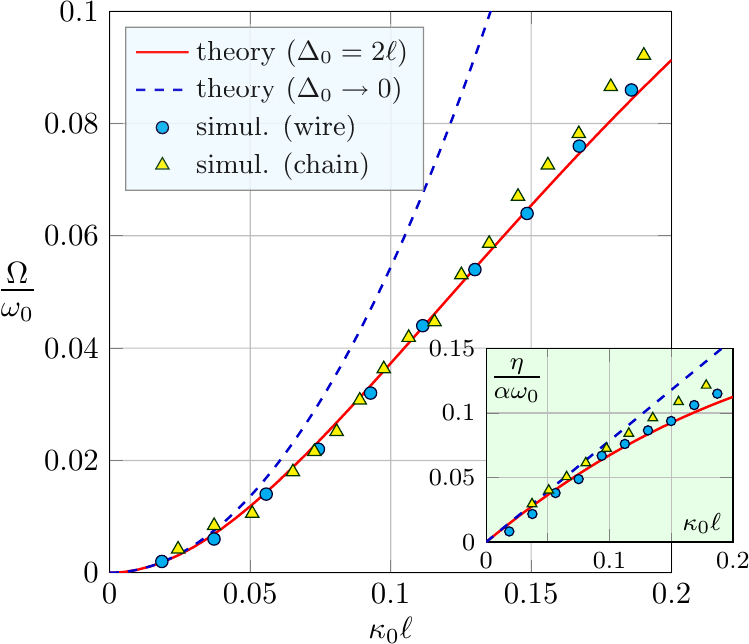
\includegraphics[width=0.5\linewidth]{DW_parabola_dynamics.png}}
	\caption{\textbf{Eigenfrequency and effective friction of the domain wall oscillations in vicinity of the equilibrium.} Solid and dashed lines correspond to the analytical predictions~\eqref{eq:Omega_eta_2}. Markers show the results of numerical simulations for nanowires (disks) and discrete chains of magnetic moments (triangles). 
	Adapted with permission from~\cite{Yershov15b}.}
	\label{fig:DW_dynamics_parabola}
\end{figure}
%==================================================================/


